\documentclass[a4paper,11pt]{article}
\usepackage{fixltx2e}
\usepackage{fullpage}
\usepackage{subfigure}
\usepackage{graphicx}

\begin{document}

\title{\bfseries Modelling a brushed DC machine}
\author{Muhammad Zaheer Naivasal, Wenzhuo Wu, Leo Zhang}
\date{December 17, 2014}
\maketitle

\section{No-load operation}
The no-load characteristics of the DC machine is given in the Fig~\ref{fig:noload} and the variation of radial flux density is given in Fig~\ref{fig:noload-brad}.
\begin{itemize}
\item Pole Flux= 0.014056 Wb
\item $T_{rotor}$= -0.01976 Nm
\item $T_{stator}$= 0.02939 Nm
\item $T_{mb}$= -0.02061 Nm
\end{itemize}

\begin{figure}[h!]
  \centering
  \subfigure[No-load characteristics of DC motor]{
    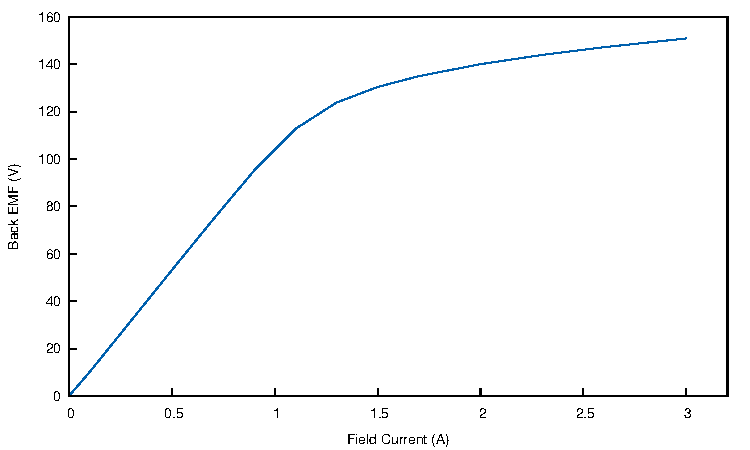
\includegraphics[scale=0.55]{noload.pdf}
%    \caption{No-load characteristics of a DC machine}
    \label{fig:noload}}
%\end{figure}
\quad
%\begin{figure}[h!]
%  \centering
  \subfigure[Radial flux density around the airgap durin no-load conditions]{
  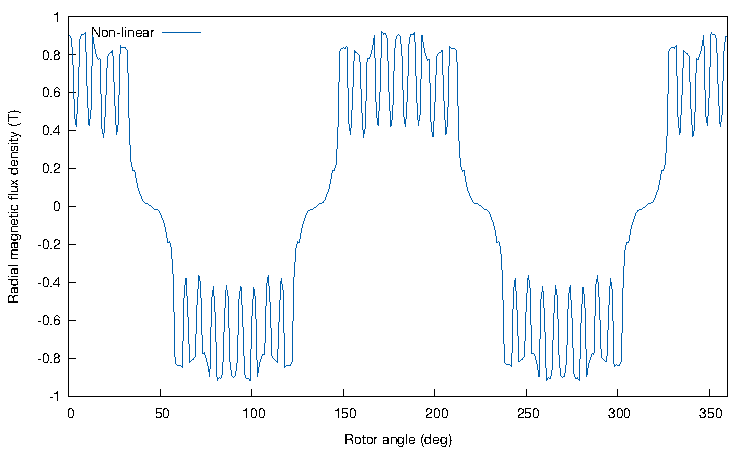
\includegraphics[scale=0.55]{noload_brad.pdf}
%  \caption{Radial Flux Density $B_{rad}$ around the airgap}
  \label{fig:noload-brad}}
  \quad
  \subfigure[Flux lines - saturation]{
    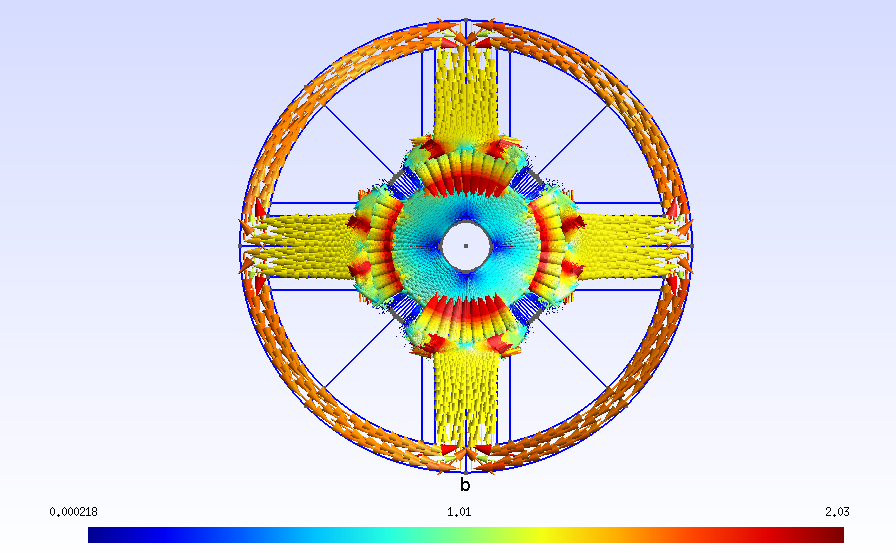
\includegraphics[scale=0.25]{No-load_NL.png}}
  \quad
  \subfigure[Flux lines - without saturation]{
    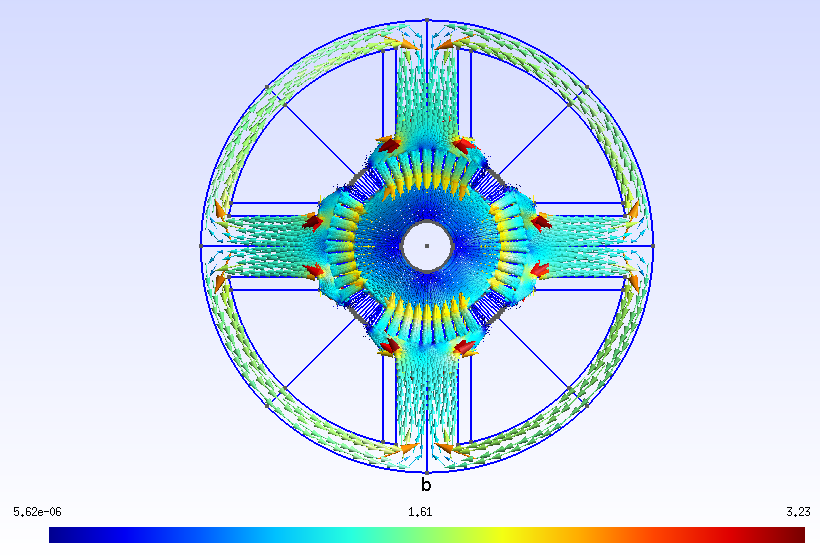
\includegraphics[scale=0.25]{No-load_L.png}}
  \caption{No-load operation of DC machine}
\end{figure}

\section{Operation with zero field current}
The variation of radial flux density around the airgap under these condition is given in the Fig~\ref{fig:nofieldnl}.

\begin{itemize}
\item Pole Flux= -6.92e-7 Wb
\item $T_{rotor}$= -0.00236 Nm
\item $T_{stator}$= 0.00934 Nm
\item $T_{mb}$= -0.00293 Nm
\end{itemize}

\begin{figure}[h!]
  \centering
  \subfigure[$B_{rad}$ around the airgap]{
  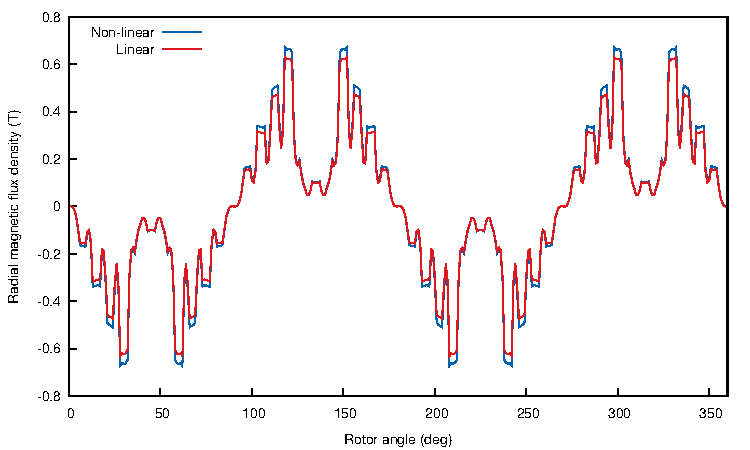
\includegraphics[scale=0.55]{nofieldNL_brad.pdf}
  \label{fig:nofieldnl}}
  \quad
  \subfigure[Flux lines - saturation]{
    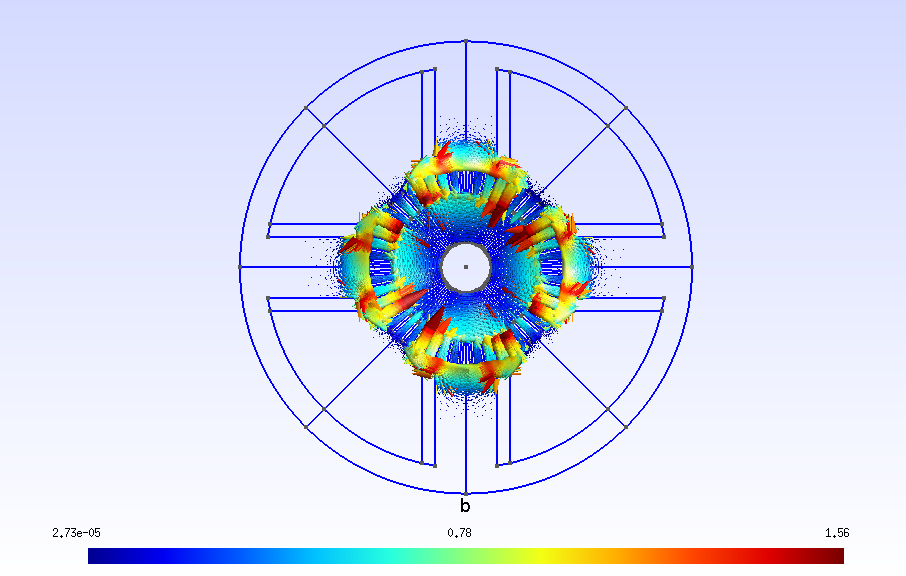
\includegraphics[scale=0.27]{No-field_NL.png}}
  \caption{Zero Field current operation}
\end{figure}

\section{Load operation}
The variation of radial flux density under different loads is given in the Fig~\ref{fig:loadnl}, Fig~\ref{fig:loadl}.

\begin{figure}[h!]
  \centering
  \subfigure[$B_{rad}$ around the airgap - saturation]{
  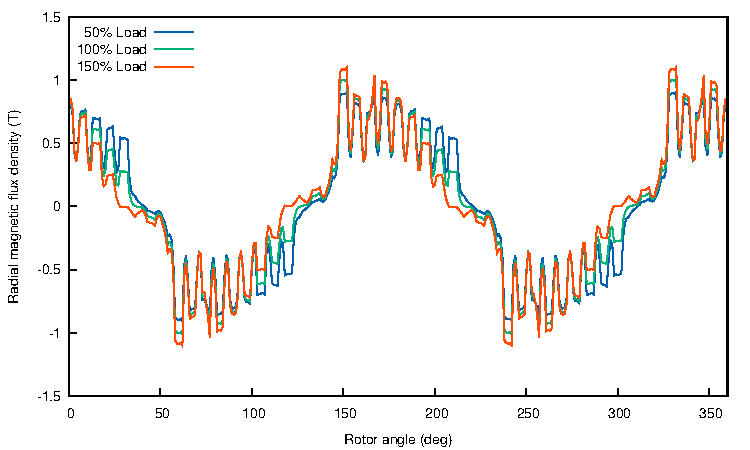
\includegraphics[scale=0.55]{load_NL_brad.pdf}
  \label{fig:loadnl}}
  \quad
  \subfigure[$B_{rad}$ around the airgap - without saturation]{
  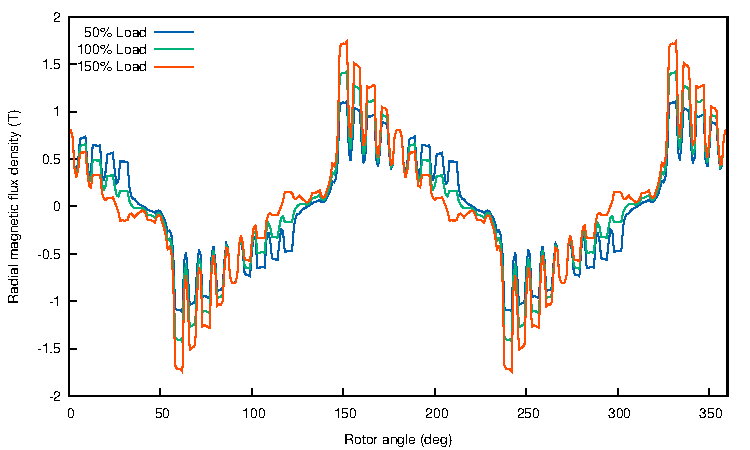
\includegraphics[scale=0.55]{load_L_brad.pdf}
  \label{fig:loadl}}
  \quad
  \subfigure[Flux lines - saturation]{
    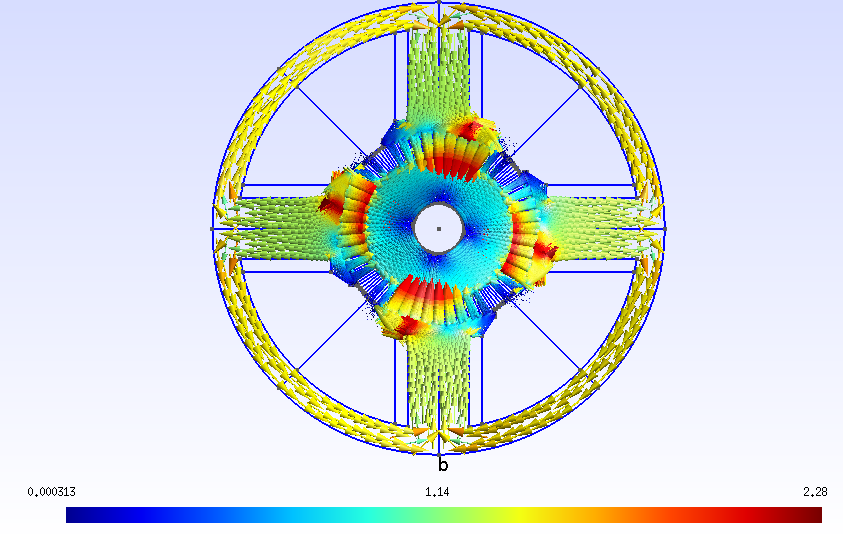
\includegraphics[scale=0.3]{Load_NL.png}}
  \quad
  \subfigure[Flux lines - without saturation]{
    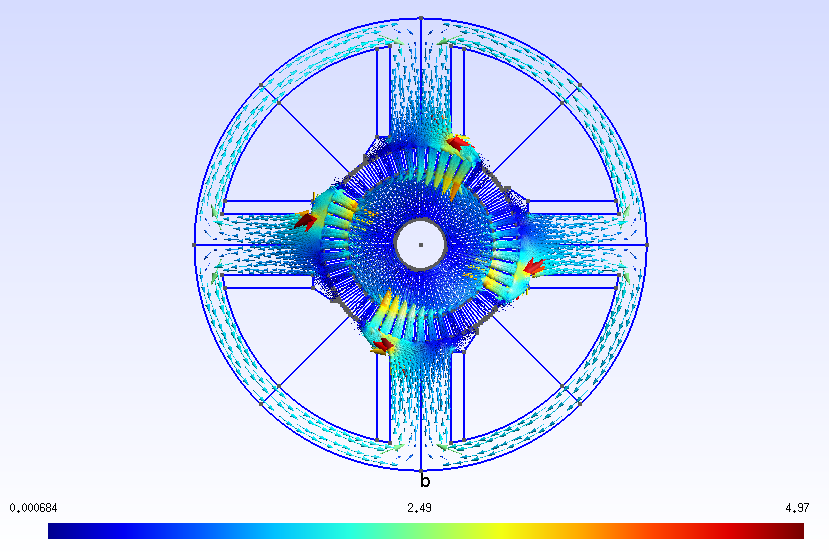
\includegraphics[scale=0.3]{Load_L.png}}
  \caption{Load operation - different loadings}
\end{figure}


\paragraph*{Pole flux computation}
The pole flux was computed using the formula given in the lab manual and the value was found to be $-4.29\times10^{-8}$Wb which is close enough to the value computed by Gmsh i.e. $-6.92\times10^{-7}$Wb

\paragraph*{Torque comparison}
According to the data of the machine given, we found the rated torque and the torque calculated by the FEM model is given in the table below
\begin{equation}
  T_{rated}=94.54 Nm
\end{equation}
\begin{center}
\begin{tabular}{|c|c|c|}
  \hline
Torque (Nm)  &  Satuaration & Without saturation \\ \hline
  T\textsubscript{rotor} & 96.0055 & 96.5586 \\ \hline
  T\textsubscript{stator} & 98.2271 & 99.616 \\ \hline
  T\textsubscript{mb} & 97.4709 & 97.9595\\ \hline
\end{tabular}
\end{center}
The differences in percent for the different torques ranges between 1-4 \%.

\paragraph*{Computation of k\textsubscript{e}}
In this case, we have considered the torque at the rotor airgap i.e. T\textsubscript{rotor} as the reference value for computing the value of \textbf{k\textsubscript{e}}. The computed values are tabulated below
\begin{center}
  Value of \textbf{k\textsubscript{e}}
  
  \begin{tabular}{|c|c|c|}
    \hline
    Loading & Saturation & Without saturation \\ \hline
    50\% & 78.9102 & 73.1843 \\ \hline
    100\% & 80.2051 & 73.1837 \\ \hline
    150\% & 81.4494 & 73.1843 \\ \hline
  \end{tabular}
\end{center}

\paragraph*{Variation of $B_{rad}$ for different field conditions}
The variation of radial flux density for different field conditions is given in Fig~\ref{fig:fieldnl} and in Fig~\ref{fig:fieldl}.

\begin{figure}[h!]
  \centering
  \subfigure[$B_{rad}$ around the airgap - saturation]{
  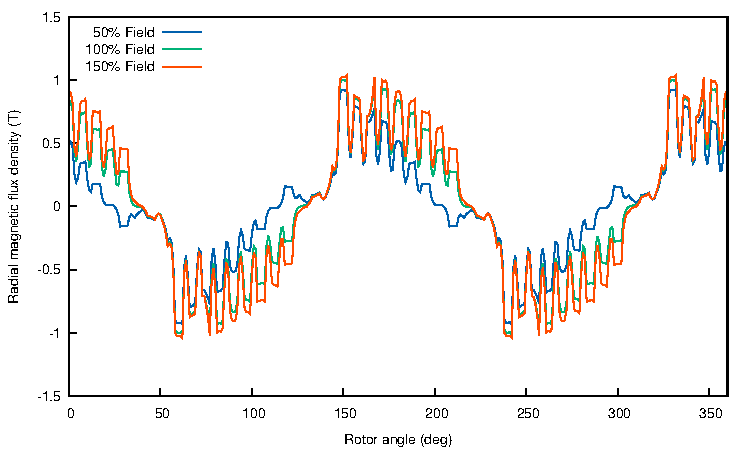
\includegraphics[scale=0.55]{field_NL_brad.pdf}
  \label{fig:fieldnl}}
  \quad
  \subfigure[$B_{rad}$ around the airgap - without saturation]{
  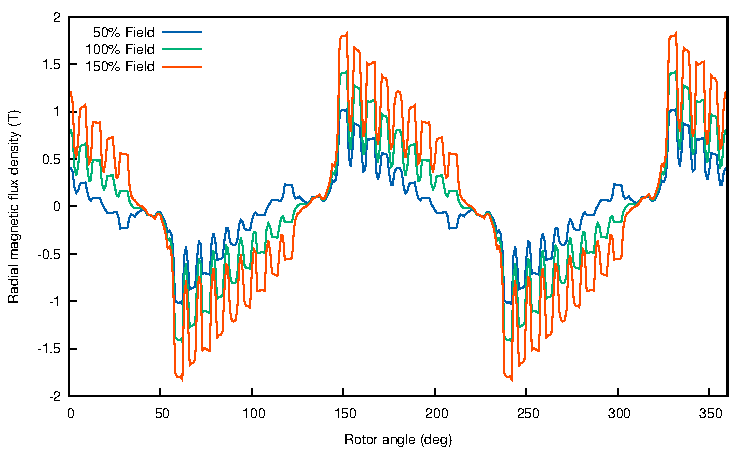
\includegraphics[scale=0.55]{field_L_brad.pdf}
  \label{fig:fieldl}}
  \caption{Load operation - different excitation conditions}
\end{figure}

\section{Other questions}
\paragraph*{Average Torque}
\begin{itemize}
\item For non-linear case T\textsubscript{avg} = 97.2345 Nm
\item For linear case T\textsubscript{avg} = 98.0447 Nm
\end{itemize}

\paragraph{When is torque null?}
Torque is proportional to the pole flux and the armature current. So, when either of them is zero then torque produced is null.

\paragraph{When is the pole flux maximum?}
The flux is at its maximum when the field current is at the maximum value and the armature current is at the minimum value as the flux is proportional to field current. However, when the machine is loaded,flux will be influenced by armature current because of the armature reaction.

\paragraph{When is the pole flux minimum?}
The flux is at its minimum when the field current is at the minimum value and the armature current is at the maximum value.

\paragraph{Symmetry}
If we have used symmetry for this model, then the smallest part of the machine that could be modelled will be half of the machine cut diagonally such that it contains two poles of the machine completely.

In such a case, the boundary conditions at the outer part of the yoke would be that the flux at that point is zero. Along the symmetrric line, the derivative of the normal component of the flux is zero. This is due to the fact that amount of flux entering one part of the rotor(symmetric line) is equal to the amount of flux leaving the other part of the rotor.
\end{document}
